%%
%% FundamentacaoTeorica.tex
%% Projeto Oficinas de Integração 3
%% Created by Leonardo Winter Pereira and Lucas Zimmermann Cordeiro on 10.03.2016
%% Copyright (C). All rights reserved
%%

\chapter{Fundamentação Teórica}
\label{chap:fundamentacaoTeorica}

    Para uma melhor compreensão e análise do funcionamento e princípios envolvidos em um controlador MIDI, é fundamental entendermos todos os conceitos nesse processo, bem como as características das tecnologias utilizadas na construção do protótipo e de ambos os aplicativos de controle. Assuntos, esses, que serão tratados no decorrer dessa seção.

    \section{MIDI}

        Uma vez que o projeto aqui proposto baseia-se, basicamente, no funcionamento deste protocolo e na troca de informações deste com outros dispositivos, é imprescindível um completo entendimento do mesmo.

        Esta será a mais longa seção deste capítulo, mas também a mais importante. Além disso, aqui serão citados grandes nomes utilizados como referência para este projeto, para o caso de o leitor se interessar pelos conteúdos aqui expostos e quiser se aprofundar nos mesmos.

        \subsection{O que é MIDI}

            O primeiro conceito que o leitor deve entender é o que é, de fato, o protocolo MIDI, citado repetidas vezes no capítulo anterior, mas que ainda não foi explicitado. Para tanto, serão citadas três definições deste e após, será estudado o real significado das mesmas.

            Adam Olson, do Conservatório Shenandoah, define MIDI como: \epigraph{[...] MIDI é um protocolo de controle que envia dados entre vários instrumentos musicais e sequênciadores.}{~\cite{McGuire}}

            Já David Miles Huber, autor do livro \textit{The MIDI Manual} define MIDI como: \epigraph{[...] Basicamente, MIDI é uma linguagem e especificação compatível de comunicação digital que permite múltiplos hardwares e softwares se comunicarem uns com os outros através de uma rede conectada.}{~\cite{Huber}}

            Robert Guérin, autor do livro \textit{MIDI Power!}, por sua vez, define MIDI como: \epigraph{[...] MIDI permite que músicos, engenheiros de som e iluminação, entusiastas da computação, ou qualquer outra pessoa usem computadores e instrumentos musicais eletrônicos para criar, ouvir e aprender sobre música, oferecendo uma linguagem comum que é compartilhado entre dispositivos e software compatíveis.}{~\cite{Guerin}}

            Com estas definições, pode-se perceber que MIDI é, por si só, incapaz de reproduzir som. Esta é sua maior qualidade. Seus dados podem ser gravados em um programa de software (conhecido como sequênciador) ou dispositivo de hardware, onde estes podem ser editados e transmitidos para instrumentos eletrônicos ou outros dispositivos para criar a música ou controlar qualquer parâmetro desejado. Além disso, MIDI pode ser separado em três entidades diferentes: A linguagem utilizada, também conhecida como protocolo de comunicação; a interface de hardware utilizada para transmitir e receber essas informações (tais como conectores e cabos); e os formatos de distribuição, tal como \sigla{SMF}{Standard MIDI Files} (Arquivos MIDI padrão). No decorrer deste capítulo, abordaremos separadamente cada entidade, a fim de entender como elas trabalham juntas e o porquê do MIDI funcionar tão bem, oferecendo interconectividade, flexibilidade e (em termos de tamanho de arquivo) portabilidade. 
            
            Fundamentalmente, MIDI é uma linguagem de descrição de música em forma binária, em que cada palavra binária descreve um evento de uma música. Cada instrumento musical realiza um som, o qual está totalmente sobre controle do músico. O músico controla o momento em que o instrumento começará a realizar um determinado som - um tecladista pressionará uma tecla, um trompetista soprará ar e um baixista puxará uma corda. Considere esta ação como o evento \textbf{Nota ON}. A mensagem MIDI em si não contém o real som tocado pelo instrumento, mas sim a ação de tocar uma determinada nota em um determinado momento e durante um determinado período.
            
            Quando o músico deixa de pressionar uma tecla em seu teclado ou de puxar uma corda em seu baixo, o som pára. Com MIDI, quando tal ação é realizada, uma mensagem é enviada para essa nota, para que esta deixe de realizar som. Esta mensagem é conhecida por \textbf{Nota OFF}. A figura ~\ref{fig:MIDI_Nota_ON_e_OFF} demonstra um exemplo destes dois eventos.
            
            \begin{figure}[!h]
            	\centering
            	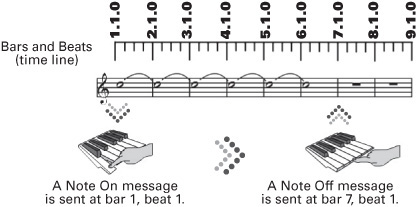
\includegraphics{Imagens/MIDI_Nota_ON_e_OFF.jpg}
            	\caption[Exemplo de transmissão das mensagens de Nota ON e OFF]{Exemplo de transmissão das mensagens de Nota ON e OFF ~\cite{Guerin}}
            	\label{fig:MIDI_Nota_ON_e_OFF}
            \end{figure}
            
            A fim de identificar qual nota foi ativada / desativada no instrumento, um número é atribuído para cada nota. MIDI também lida com valores interpretativos, como por exemplo a velocidade que a nota foi pressionada e a pressão que é executada na mesma.
            
        \subsection{O protocolo de comunicação MIDI}
        
            O protocolo de comunicação MIDI é transmitido de forma serial ao invés de paralela. Em uma transmissão paralela, como o nome sugere, as informações são transmitidas simultaneamente. A quantidade de dados que podem ser transmitidos simultaneamente depende na capacidade física do fio e da velocidade com que os dispositivos podem enviar suas informações. Na figura ~\ref{fig:Parallel_versus_serial_transmissions}, podemos perceber que um \textit{byte} (oito \textit{bits}) é transmitido simultaneamente utilizando uma transmissão paralela. A transmissão serial, por outro lado, consegue enviar apenas um \textit{bit} após o outro.
            
            \begin{figure}[!h]
            	\centering
            	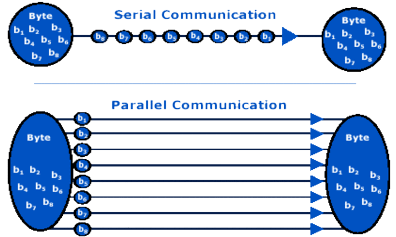
\includegraphics[scale=0.8]{Imagens/Parallel_versus_serial_transmissions.png}
            	\caption[Comparação entre transmissão serial e paralela]{Comparação entre transmissão serial e paralela}
            	\label{fig:Parallel_versus_serial_transmissions}
            \end{figure}
            
            A pergunta que fica é: Por que MIDI usa transmissão serial ao invés da transmissão paralela?

            A resposta para essa pergunta está no período em que o protocolo foi desenvolvido. A transmissão paralela tinha algumas desvantagens que superavam as vantagens desta sobre a transmissão serial, além de ser muito mais cara, uma vez que os fios, conectores e tomadas eram mais complexos. Já a transmissão serial, por outro lado, era muito mais simples de ser produzida, mais acessível para o público e rápida o suficiente para os fins que os fabricantes e usuários tinham em mente naquela época, para não mencionar mais confiável. Com o passar dos anos, a tecnologia avançou muito e os custos da transmissão paralela despencaram. Entretanto, para manter o MIDI compatível com todos os antigos dispositivos, sua forma de transmissão de dados permaneceu inalterada desde sua introdução no mercado.
            
            MIDI envia informação a uma taxa de 31250 \sigla{bps}{\textit{bits} por segundo}. Essa velocidade é chamada de taxa de transmissão. Uma vez que o protocolo utiliza transmissão serial, o mesmo envia apenas um \textit{bit} por vez. Cada \textit{byte} em uma mensagem MIDI contém 10 \textit{bits} de dados (8 \textit{bits} para as informações e 2 \textit{bits} para correção de erro). Isso significa que MIDI envia cerca de 3125 \textit{bytes} de dados cada segundo.
            
            Quando comparamos esse valor com a taxa de transmissão de 176400 \textit{bytes} necessária para transmitir áudio digital (reprodução e gravação) em formado de CD de áudio, MIDI pode parecer incrivelmente devagar. Entretanto, neste último não é necessário enviar tanta informação quanto o áudio digital, sendo capaz de, teoricamente, transmitir até 500 mensagens MIDI por segundo. Na realidade, leva cerca de um milésimo de segundo para transmitir uma única nota. O limiar para distinguir os eventos de som individuais é de aproximadamente 10 milissegundos, então você apresentará dificuldades com 10 ou mais eventos simultâneos.
        
        \subsection{Hardware e conectores}

            Informações MIDI são transmitidas através de fios e conectores, e seus cabos podem apresentar até 15 metros de comprimento. Entretanto, por se tratar de um cabo serial, todos os dados são transmitidos através de um único fio principal, e grandes distâncias podem inferir em uma degradação do sinal, ocasionando em possíveis perdas de dados ou mensagens impossíveis de serem lidas.
            
            \begin{figure}[!h]
            	\centering
            	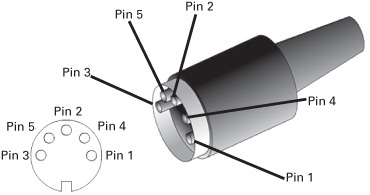
\includegraphics[scale=0.8]{Imagens/MIDI_connector.jpg}
            	\caption[Conector MIDI]{Conector MIDI}
            	\label{fig:MIDI_connector}
            \end{figure}
        
            \subsubsection{MIDI OUT}



            \subsubsection{MIDI IN}



            \subsubsection{MIDI THRU}
        


        \subsection{Formatos de distribuição}
        
        
        
    \section{Microcontroladores e Arduino}



        \subsection{Microcontroladores}



        \subsection{Arduino}

